\documentclass[12pt]{article}
\usepackage[utf8x]{inputenc}
\usepackage[spanish]{babel}
\usepackage{url}
\usepackage{cancel}
\usepackage{lipsum}
\usepackage{graphicx}
\usepackage{caption}
\usepackage{subcaption}
\usepackage{tabularx}
\usepackage{booktabs}
\usepackage{threeparttable}
\usepackage{color}
\usepackage{float}
\usepackage{amsmath}
\usepackage{listings}
\usepackage{amssymb}
\usepackage{listings}
\usepackage{geometry}
\usepackage{pythonhighlight}
\usepackage{tikz}
\geometry{
	letterpaper,
	total={170mm,240mm},
	left=20mm,
	top=20mm,
}

\title{
	\vspace{-25mm}\begin{figure}[h]
		\centering
		
\includegraphics[width=1in]{Escudo_de_la_Universidad_Nacional_de_Colombia.png}
		\label{escudo}
	\end{figure}
	Aplicaciones de elementos finitos\\
	\Large Universidad nacional de Colombia\\ 
	Facultad de ingeniería }

\author{Jhon Sebastian Gómez Castillo -
 \textit{jsgomezca@unal.edu.co}
}

\begin{document}
\maketitle
\section{Esquemas de integración temporal}  \label{esquemas}
\subsection{Integración exponencial}
La integración exponencial basada en sub espacios de Krylov se busca aproximar la matriz exponencial de un problema de ecuaciones diferenciales ordinarias (\ref{linear problem}) con condiciones iniciales (\ref{initial condition} con un espacio de menor dimensión 

\begin{equation}
	\frac{d \mathbf{u}(t)}{dt} = \mathbf{A} \mathbf{u}(t) + \mathbf{q}(t)
	\label{linear problem}
\end{equation}
\begin{equation}
	\mathbf{u}(0) = \mathbf{v}
	\label{initial condition}
\end{equation}

Para una matriz del sistema $\mathbf{A}$ un vector de valores nodales $\mathbf{u}$,  unas condiciones iniciales $\mathbf{v}$ y unos términos fuente $\mathbf{q}$ Las soluciones del sistemas estarán dadas de la siguiente forma \cite{schulze}.

\begin{equation}
	\mathbf{u}(t) = e ^{t \mathbf{A}} \mathbf{v} + \int_0 ^t e^{(t-s)\mathbf{A}} \mathbf{q}(s) ds
\end{equation}

\subcaption{Integrador exponencial y el El metodo de los elementos finitos}

Podemos usar el método de integración exponencial para poder resolver problemas en estado transitorio uno de los problemas mas sensillos de este tipo de problemas es el problema de flujo de calor en estado trancitorio (\ref{Heat transitory}) el cual se ocupara como ejemplo para demostrar como implementar el metodo de integración exponencial y el metodo de los elementos finitos:  \\


\begin{equation}
	\frac{\partial u}{\partial t}-\nabla^2 u =f  \ \ \ x \in (\Omega) \ \  y \ \ t \in (0,T]
	\label{Heat transitory}
\end{equation}

Con condiciones de frontera :

\begin{align}
	u &= u_D &en \ \Omega \times( 0,T]   \\
	u&=u_0 &en \ \Omega \times (0,T] 
\end{align}
El primer paso consiste en discretizar espacial mente el problema de Ecuaciones diferenciales parciales mediante el método de los elementos finitos. Por lo que formulamos la forma débil del problema para las funciones base $u$ y la función de prueba $v$ integrando en dominio $\Omega$ 
\begin{equation}
	\int_\Omega \frac{\partial u}{\partial t}v dx  -\int_\Omega (\nabla^2 u)v dx = \int_\Omega fv dx 
\end{equation}

Aplicando el teorema de la divergencia tenemos que: 
\begin{equation}
	\int_\Omega \frac{\partial u}{\partial t}v dx  \int_\Omega\nabla u\cdot\nabla v dx - \int_{\partial\Omega}{\partial u\over
		\partial n}v ds = \int_\Omega fv dx 
\end{equation}

Así pues nuestro problema variacional sera: \\

Encontrar un $u \in V$ tal que:  
\begin{equation}
	\int_\Omega \frac{\partial u}{\partial t}v dx  \int_\Omega\nabla u\cdot\nabla v dx - \int_{\partial\Omega}{\partial u\over
		\partial n}v ds = \int_\Omega fv dx  \ \ \ \ \  \forall v \in \hat{V}
\end{equation}

Definiendo los espacios $V$ y $\hat{V}$ como : 
\begin{align}
	V      &= \{v \in H^1(\Omega) : v =u_D  \mbox{ en } \partial\Omega\}, \\ 
	\hat{V} &= \{v \in H^1(\Omega) : v = 0 \mbox{ en } \partial\Omega\}
\end{align}

La discretización de las incógnitas y funciones de prueba se realiza a través de elementos finitos conformes en una malla $\mathcal{T}_h$, donde $h$ representa el tamaño característico del elemento. La malla $\mathcal{T}_h$ divide el dominio $\Omega$ en subdominios más pequeños, generalmente triángulos o tetraedros en geometrías tridimensionales. Cada elemento de la malla se denota como $\Omega_e$


\subsection{esquemas BDF }
Para contrastar el método de integración temporal con otros métodos de alto orden en la integración temporal usaremos los esquemas BDF para aproximar la derivada temporal del problema variacional.\\
 
Los esquemas de discretizacion  BDF, conocidos como Backward Differentiation Formulas. Estas discretizaciones son particularmente útiles cuando se busca una aproximación de segundo orden en el tiempo. En esencia, las BDF de segundo orden emplean una combinación ponderada de los valores actuales y previos de las variables para calcular las derivadas temporales en un instante futuro. Esto se logra mediante una fórmula recursiva que utiliza pasos temporales anteriores para estimar el valor en el siguiente paso. Matemáticamente, para una variable $u$ y un intervalo de tiempo discreto $\Delta t$, una discretización de la familia BDF se expresa como:
\begin{equation}
	\frac{\partial u}{\partial t} \approx \frac{\beta_0}{\gamma \Delta t} u(t^n) + \sum_{i = 1}^{s} \frac{\beta_i}{\gamma \Delta t} u (t^{n-i}) 
\end{equation}
donde $u^n = u(t^n)$ representa el valor de la variable en el tiempo discreto $n\Delta t$.
Cada uno de los coeficientes para cada esquema están dados en la Tabla \ref{tabla2}.

% Please add the following required packages to your document preamble:
% \usepackage{booktabs}
\begin{table}[!h]
	\label{tabla2}
	\caption{Coeficientes para los métodos BDF.}
	\centering
	\begin{tabular}{@{}llllll@{}}
		\toprule
		Esquema                & $\gamma$ & $\beta_0$ & $\beta_1$ & $\beta_2$ & $\beta_3$ \\ \midrule
		BDF1 (Euler implicito) & 1     & 1       & -1      &         &         \\
		BDF2                   & 2     & 3       & -4      & 1       &         \\
		BDF3                   & 6     & 11      & -18     & 9       & -2      \\ \bottomrule
	\end{tabular}
\end{table}
\section{Casos de prueba}
Se eligieron dos casos como Benchmark para probar el desarrollo computacional implementado. el primero es eun problema de pulso gausiano rotatorio y el segundo es un problema de conducción unidimensional con condición de neumman 


%graficar   (L2(x,t) o max(L2(x)) vs cpu time )\\
%graficar (L2(x)vs H_m fijo )


\subsection{Pulso gausiano}

Sea el problema de ecuaciones diferenciales parciales definido por : 

\begin{equation}
	\frac{\partial u}{\partial t} - 0.0001 \nabla  u + \nabla \cdot (w u)=0 \text{en} \  M=\Omega \times (0,T) 
	\label{pulse}
\end{equation}

Donde:  
\begin{align}
	&u(x,t) \in \mathbb{R}\\
	&\Omega = {x \in \mathbb{R}^2 : x_i \in (-0.5,0.5), i=1,2 }\\
		&w(x_1,x_2) = [-4x_2,4x_1] \\
		&T= \frac{\pi}{2}
\end{align}

podemos escribir el problema variacional para un espacio discreto de la ecuación como : \\

Encuentre un $u \in V$ tal que:  
\begin{equation}
\int_\Omega \frac{\partial u}{\partial t}v dx + 0.0001\int_\Omega\nabla u\cdot\nabla v dx  + \int _\Omega (\nabla \cdot wu)v dx  = 0 \ \ \ \ \  \forall v \in \hat{V}
\end{equation}

\subsubsection{Resultados}
\begin{figure}
	\centering
	\begin{subfigure}[b]{0.3\textwidth}
		\centering
		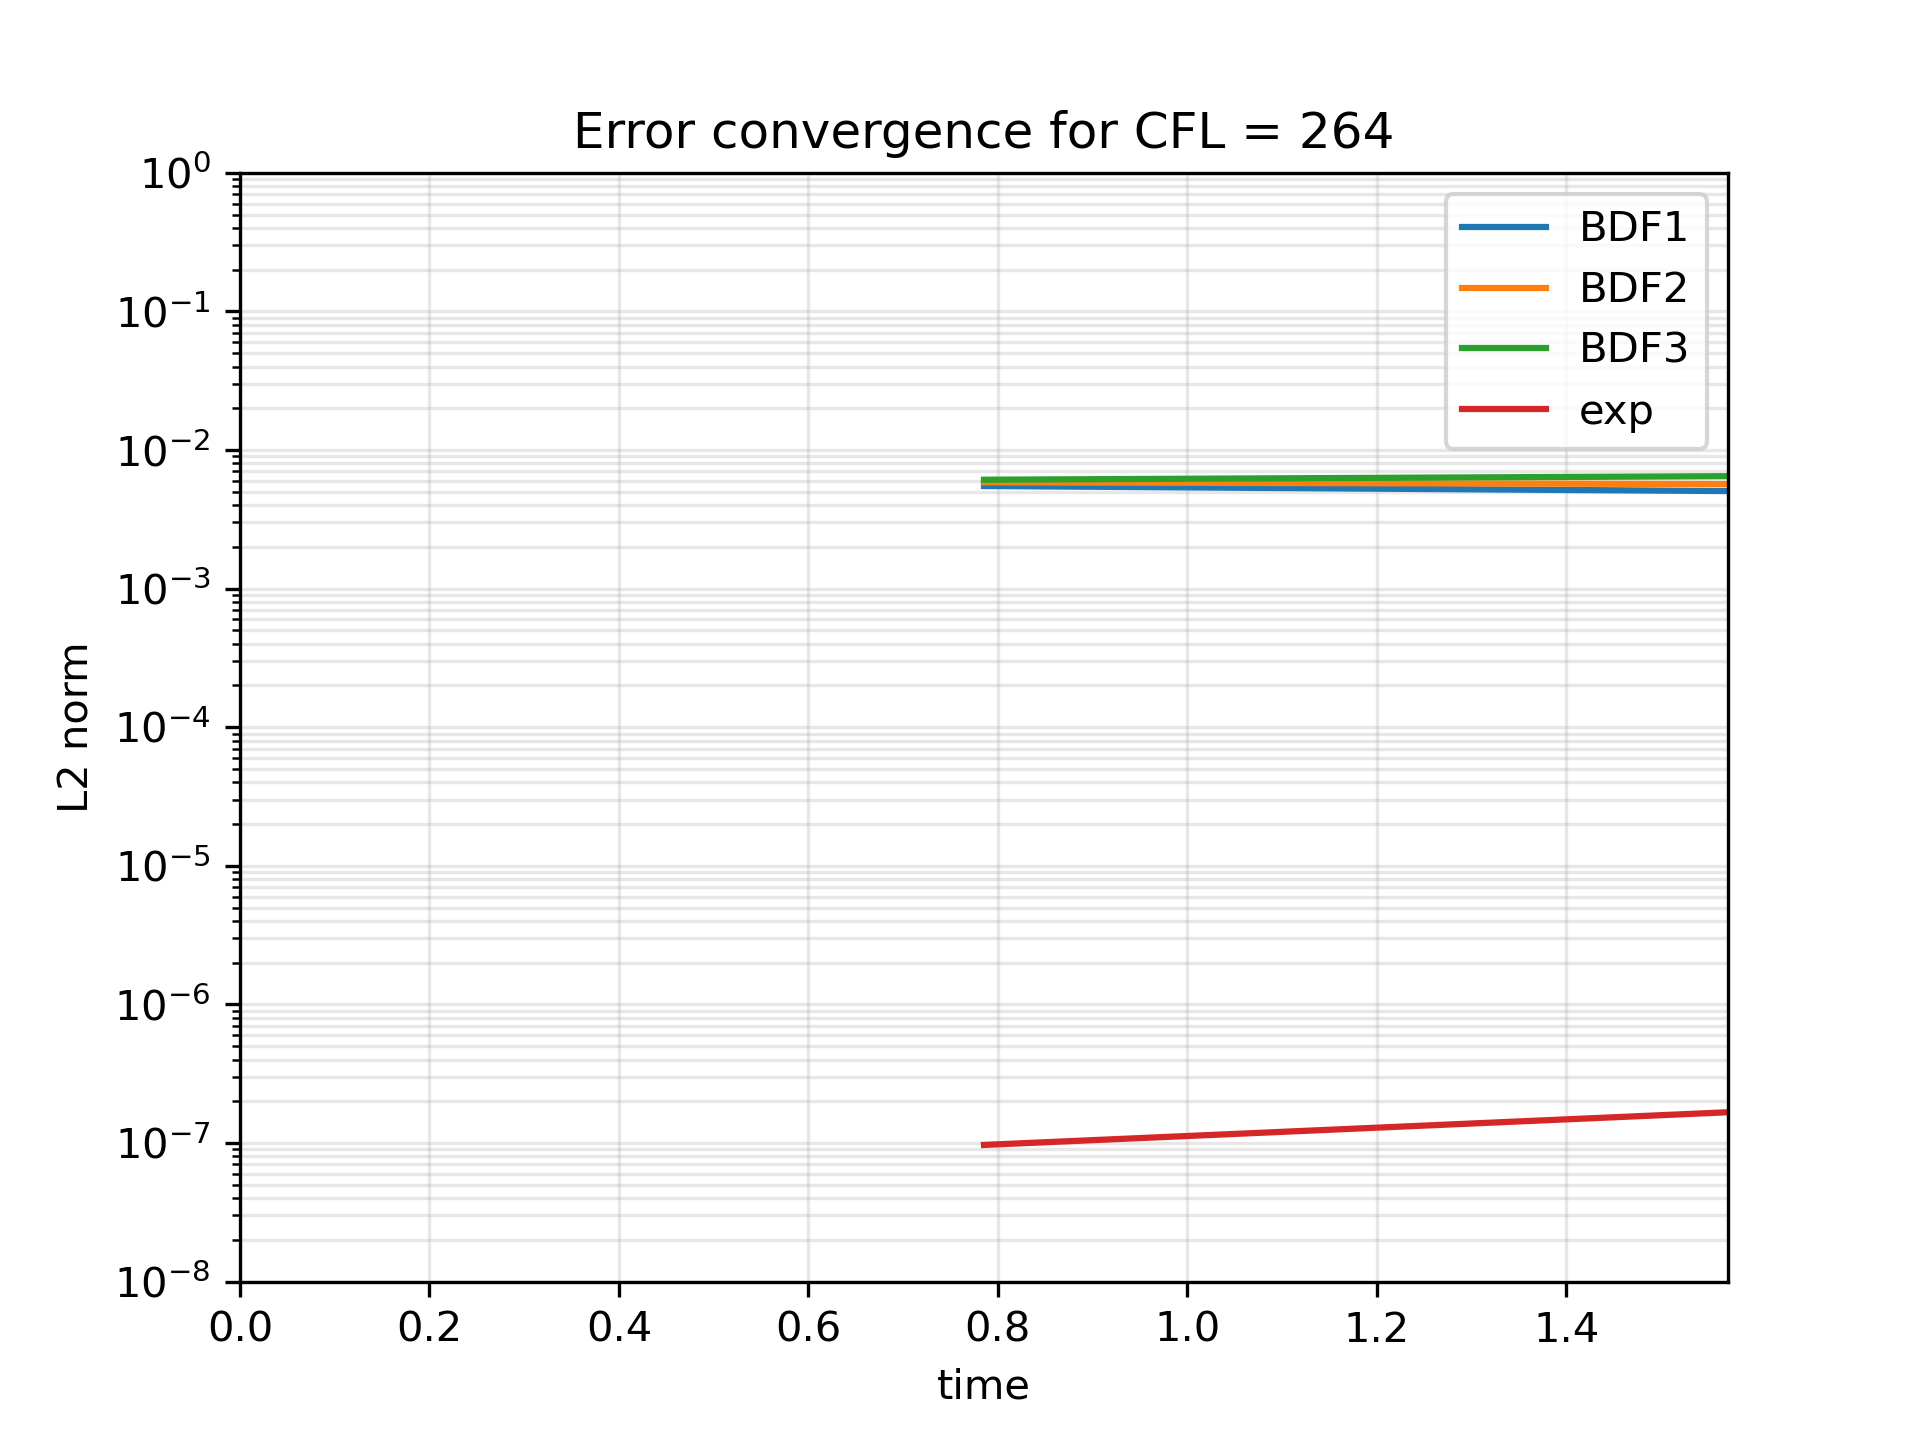
\includegraphics[width=0.7\linewidth]{res/homogeneo/L2norm_CFL_264}
		\caption{CFL 264}
		\label{fig:l2normcfl264}
	\end{subfigure}
	\begin{subfigure}[b]{0.3\textwidth}
		\centering
		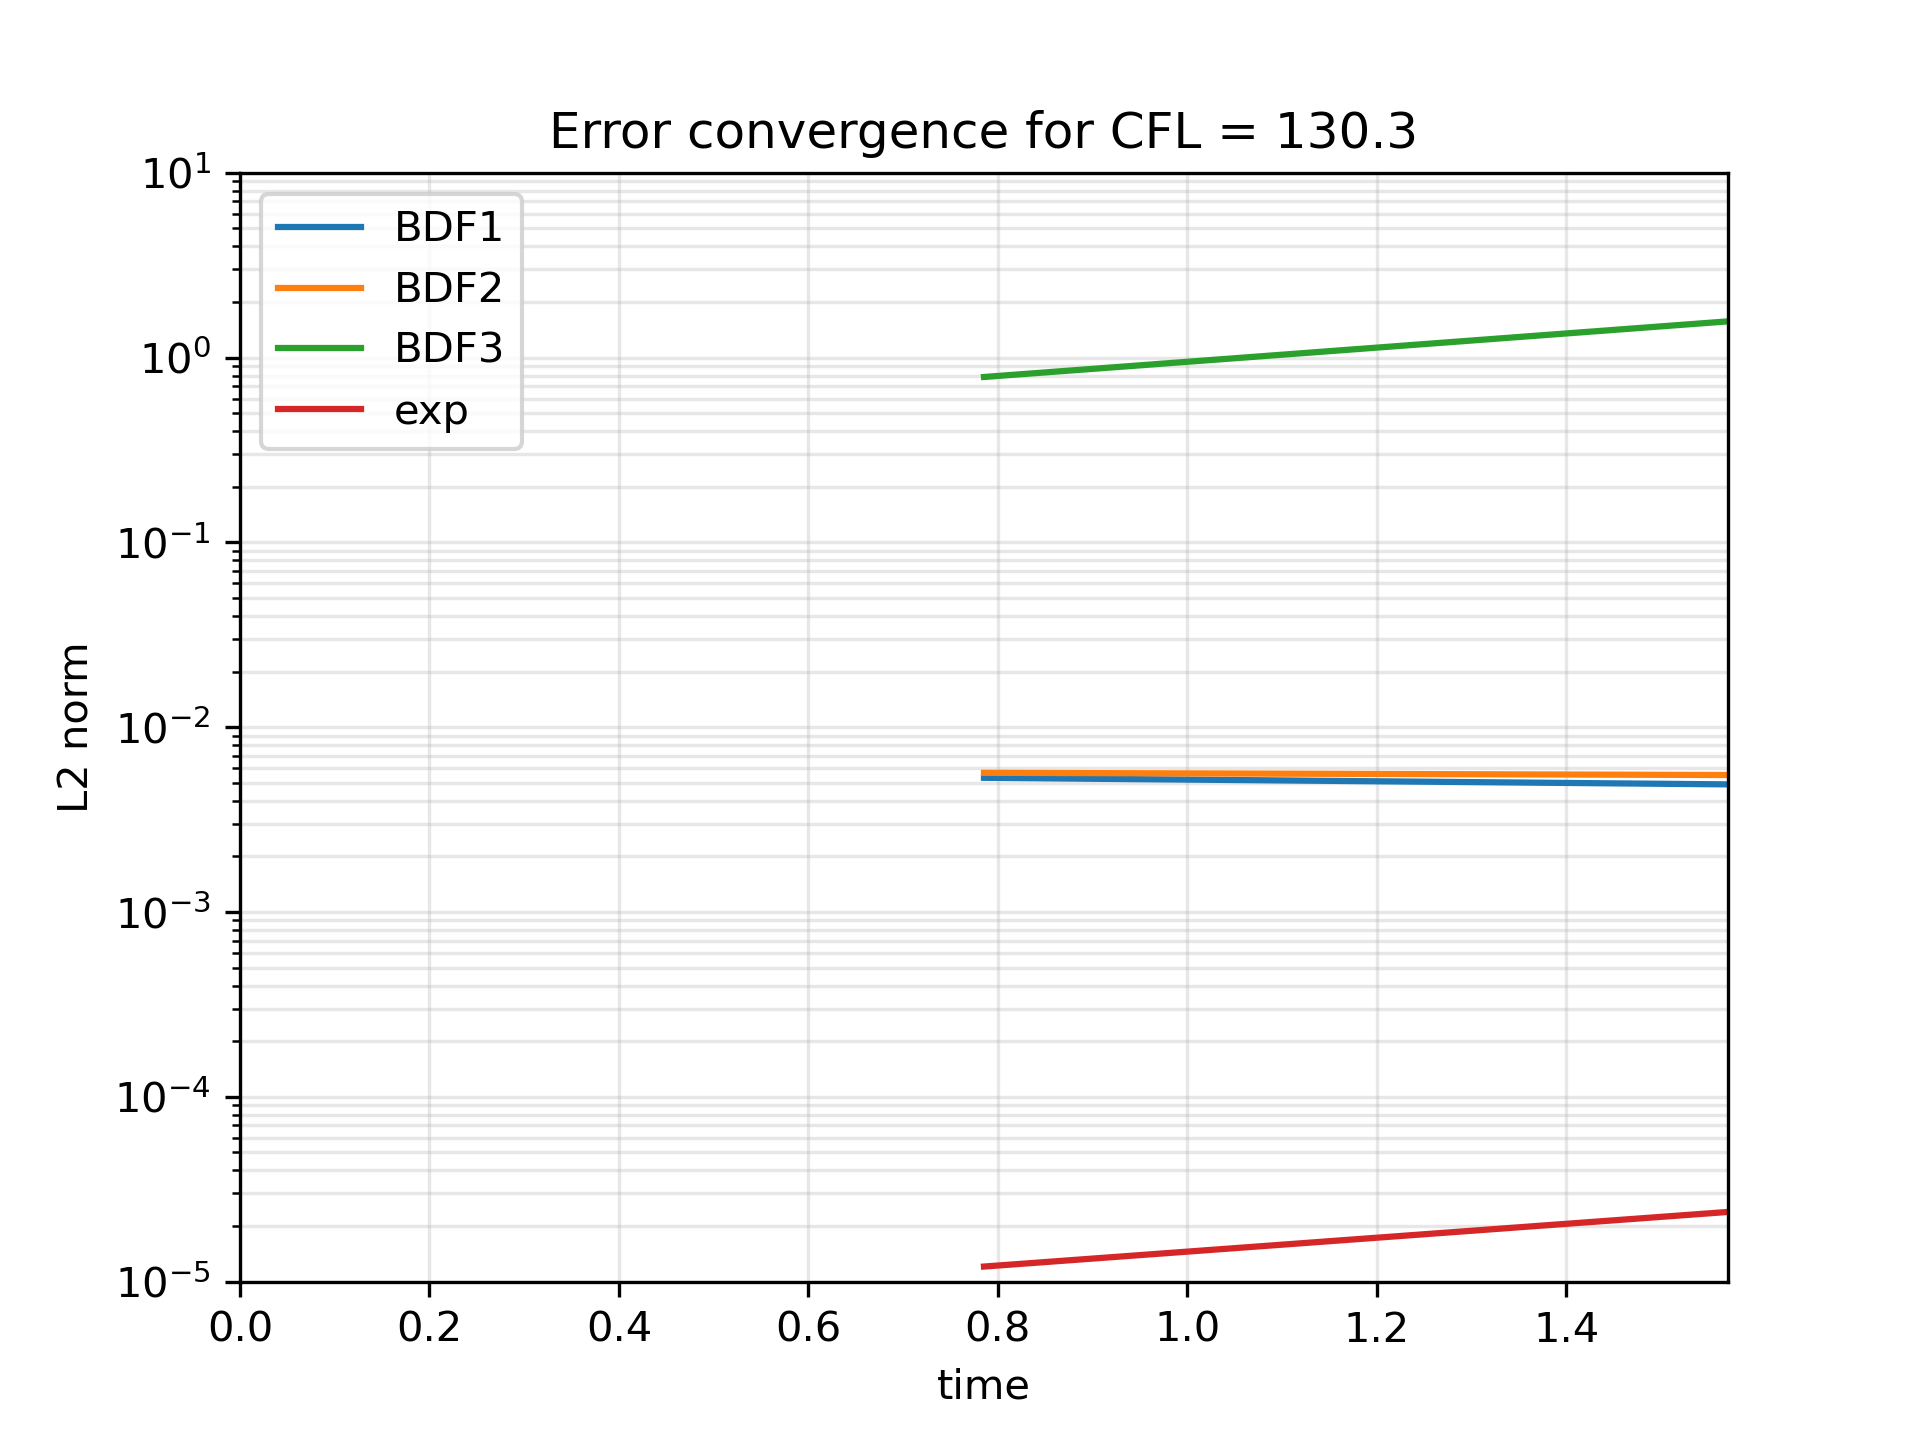
\includegraphics[width=0.7\linewidth]{res/homogeneo/L2norm_CFL_130.3}
		\caption{cfl 130.3}
		\label{fig:l2normcfl130}
	\end{subfigure}
	\begin{subfigure}[b]{0.3\textwidth}
		\centering
		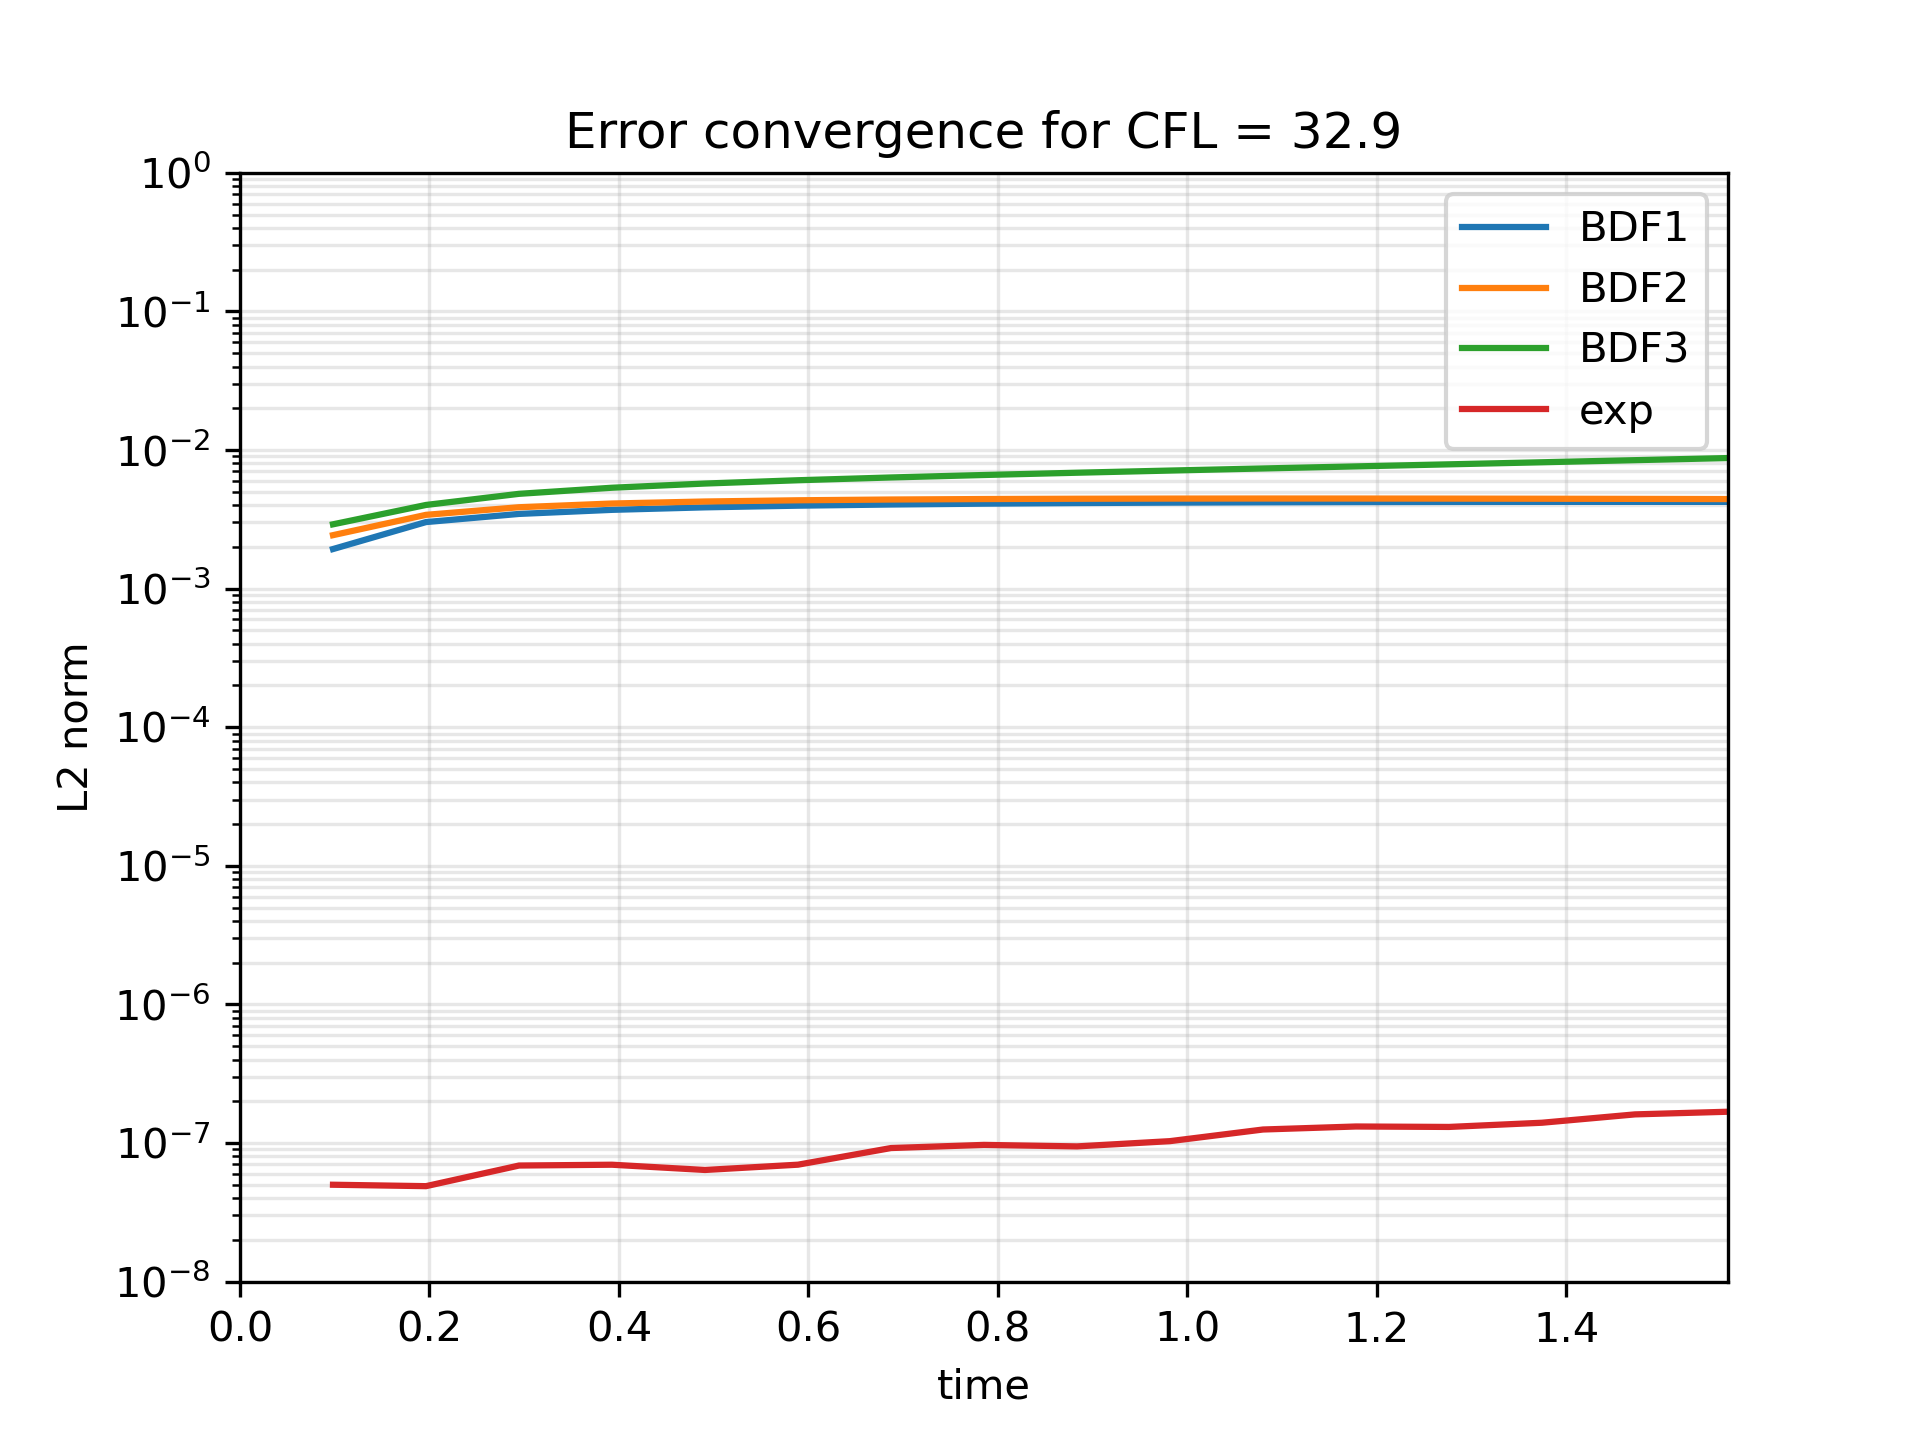
\includegraphics[width=0.7\linewidth]{res/homogeneo/L2norm_CFL_32.9}
		\caption{32.9}
		\label{fig:l2normcfl32}
	\end{subfigure}
	\begin{subfigure}[b]{0.3\textwidth}
		\centering
		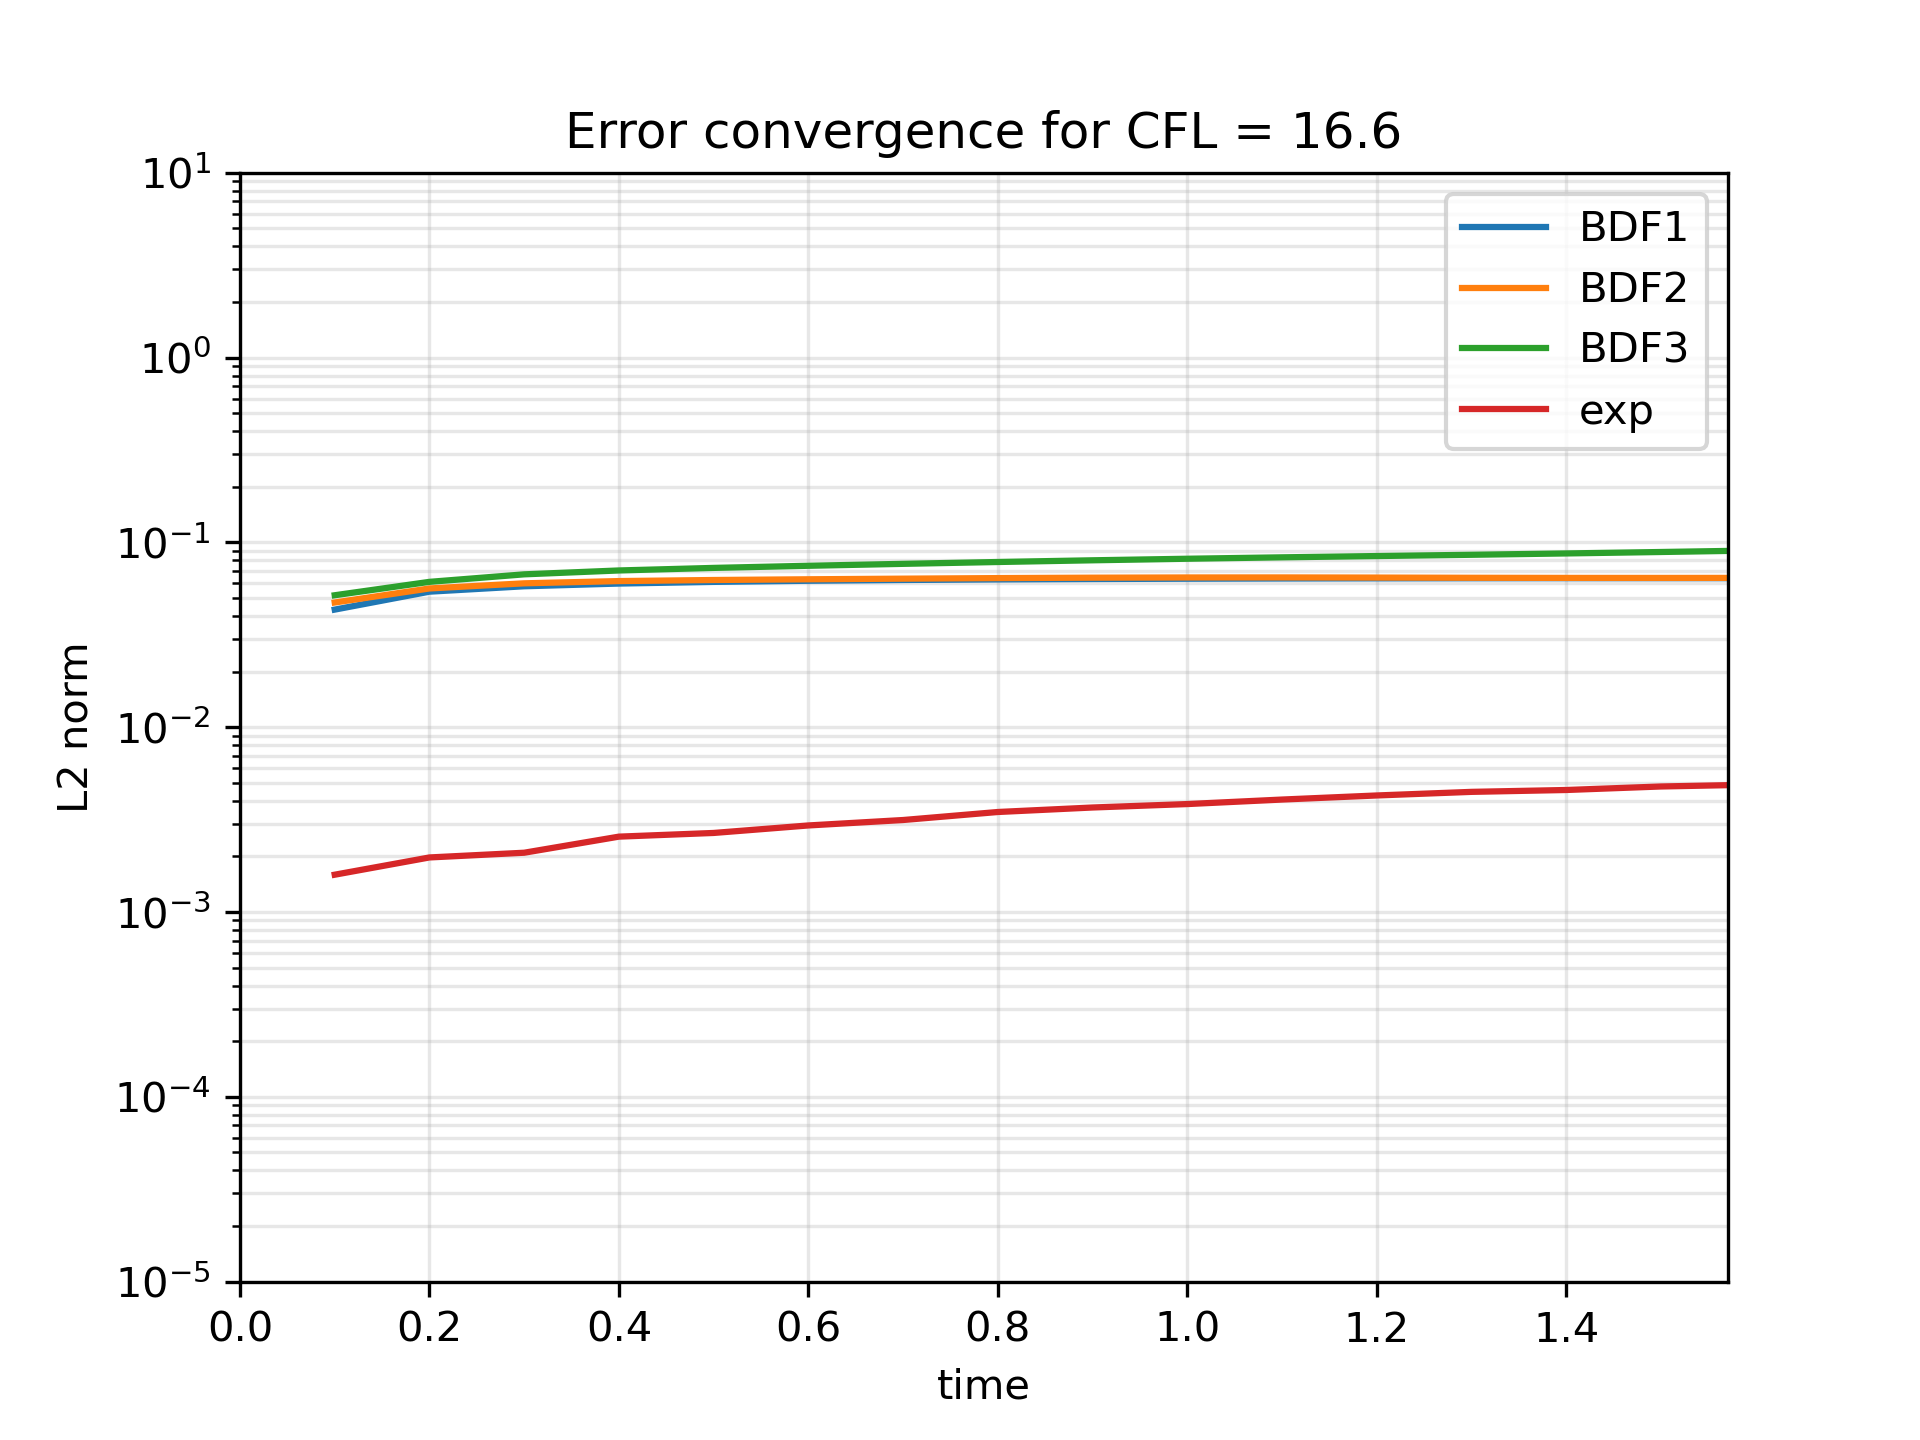
\includegraphics[width=0.7\linewidth]{res/homogeneo/L2norm_CFL_16.6}
		\caption{cfl 16.6}
		\label{fig:l2normcfl16}
	\end{subfigure}
	\caption{Three simple graphs}
	\label{fig:three graphs}
\end{figure}









\subsection{Flujo de calor }
Se escogió un problema con condiciones de frontera no homogéneas tal que el sistema linear que representa el problema discretizado tampoco es homogéneo asi pues el problema de ecuaciones diferenciales parciales es : 


\begin{align}	\frac{\partial u\left(  x,t\right)  }{\partial t}  & =\frac{\partial^{2}u(  x,t) }{\partial x^{2}}
\end{align}
con las condiciones de frontera y condición inicial  : 
\begin{align}
	\frac{\partial u}{\partial x}\left(  0,t\right)    & =1\\
	u\left(  L,t\right)    & =25\\
	u\left(  x,0\right)    & =25
\end{align} 

El problema tendrá una solución analítica dada por series  tal que : 

\begin{equation}
	u(x,t)  =x+24+\sum_{n=1}^{\infty}\frac{8}{\left(  1-2n\right)
		^{2}\pi^{2}}\cos\left(  \left(  n-\frac{1}{2}\right)  \pi x\right)
	e^{-\left(  \left(  (n-\frac{1}{2})\right)  \pi\right)  ^{2}t}
\end{equation}

La discretización se realiaza conforme a lo explicado en la sección \ref{esquemas}  

\subsubsection{Resultados }
\begin{figure}
	\centering
	\begin{subfigure}[b]{0.4\textwidth}
		\centering
		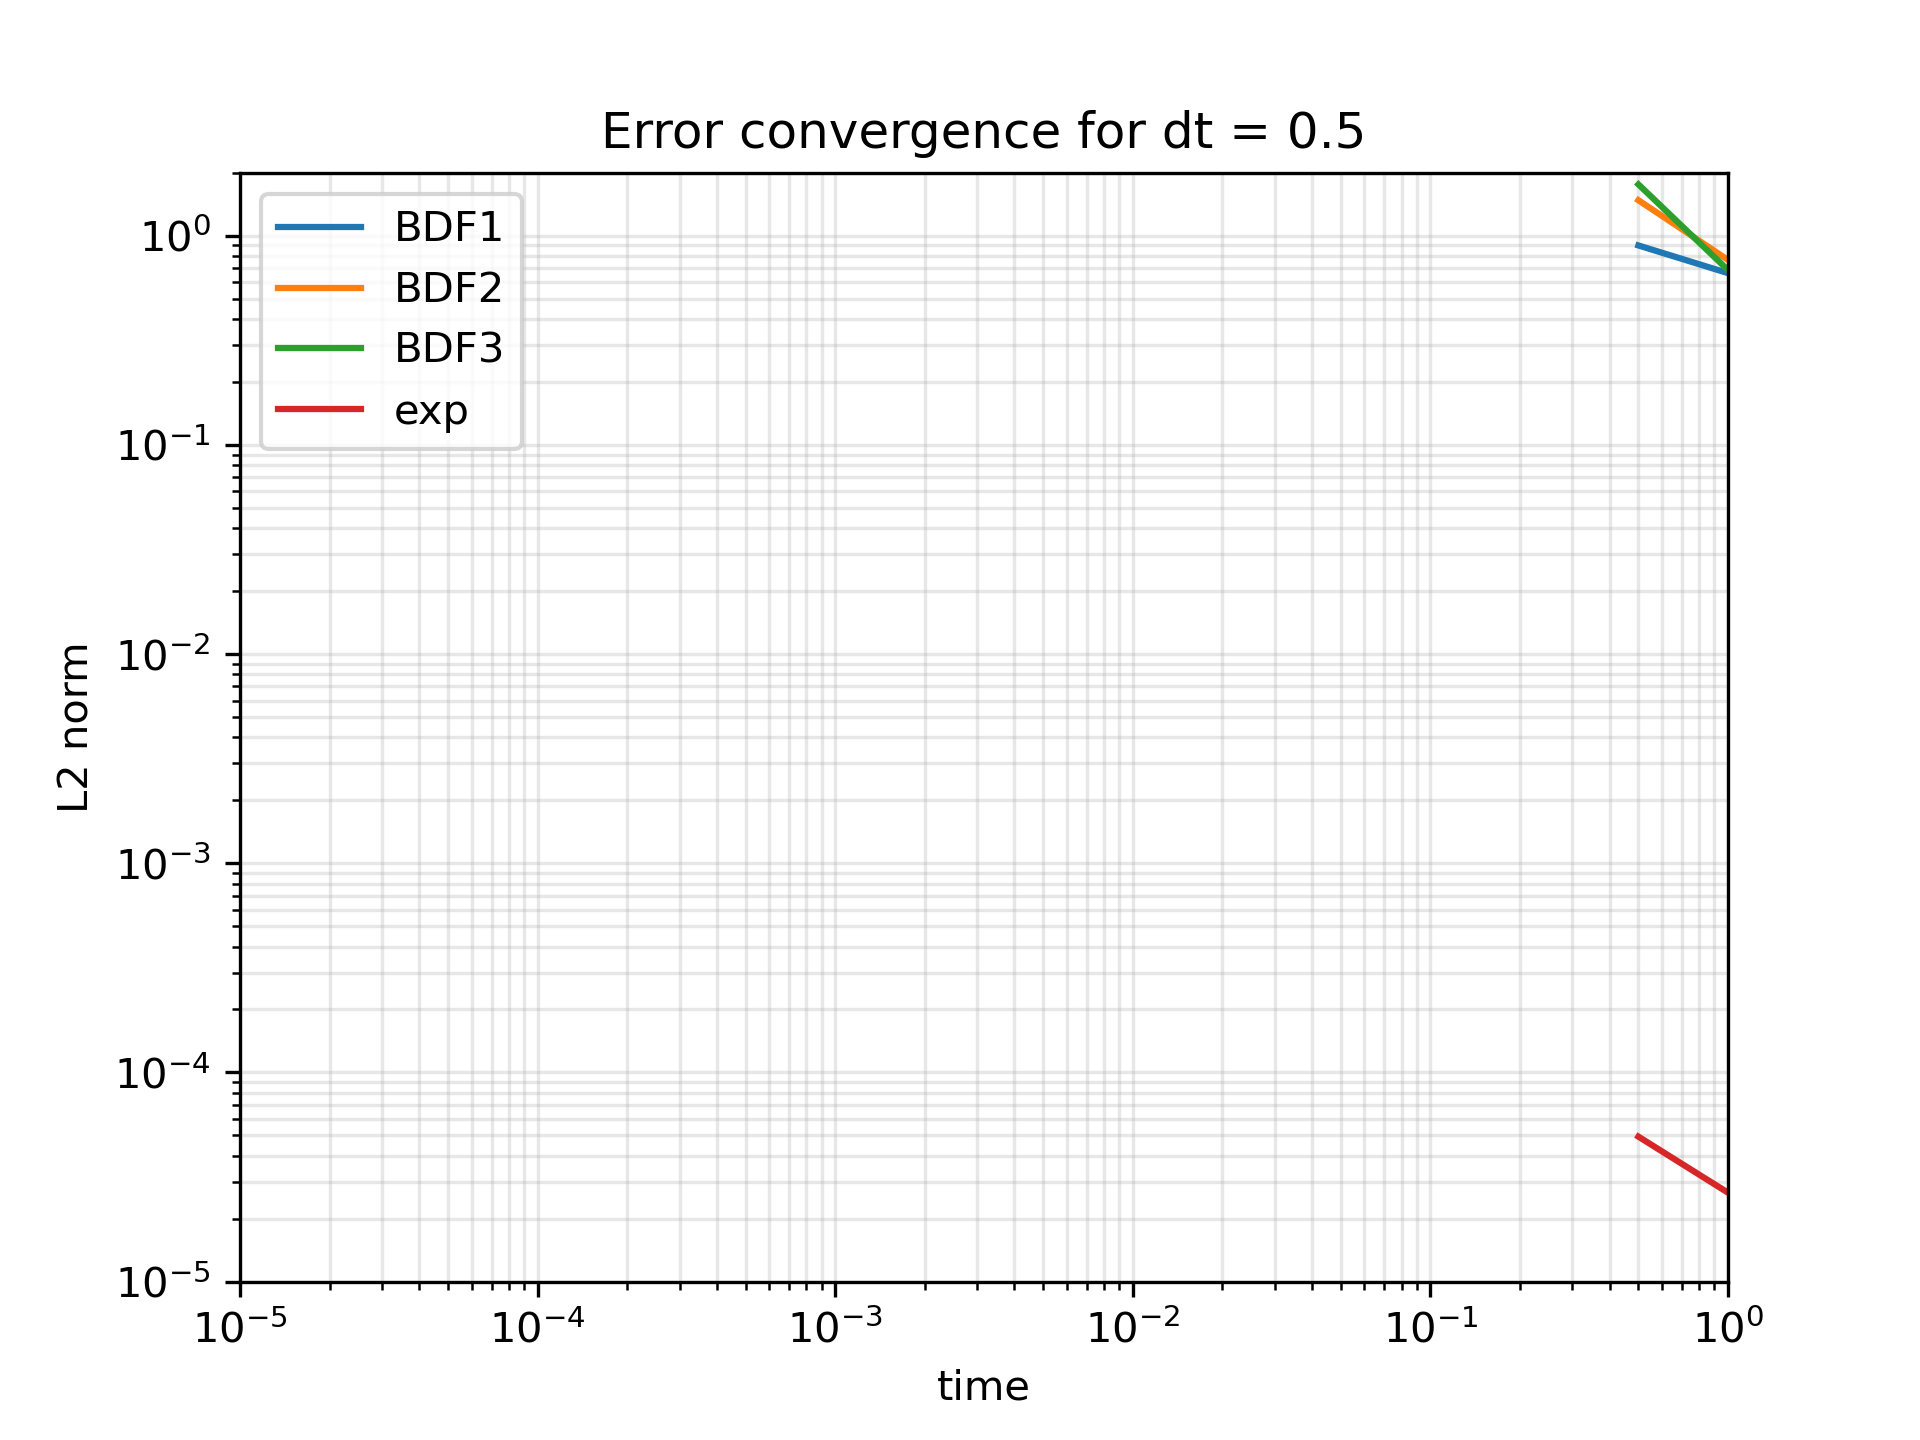
\includegraphics[width=0.7\linewidth]{res/no_homogeneo/L2norm_dt_0.5}
		\caption{}
		\label{fig:l2normdt0.5}
	\end{subfigure}
	\begin{subfigure}[b]{0.4\textwidth}
		\centering
		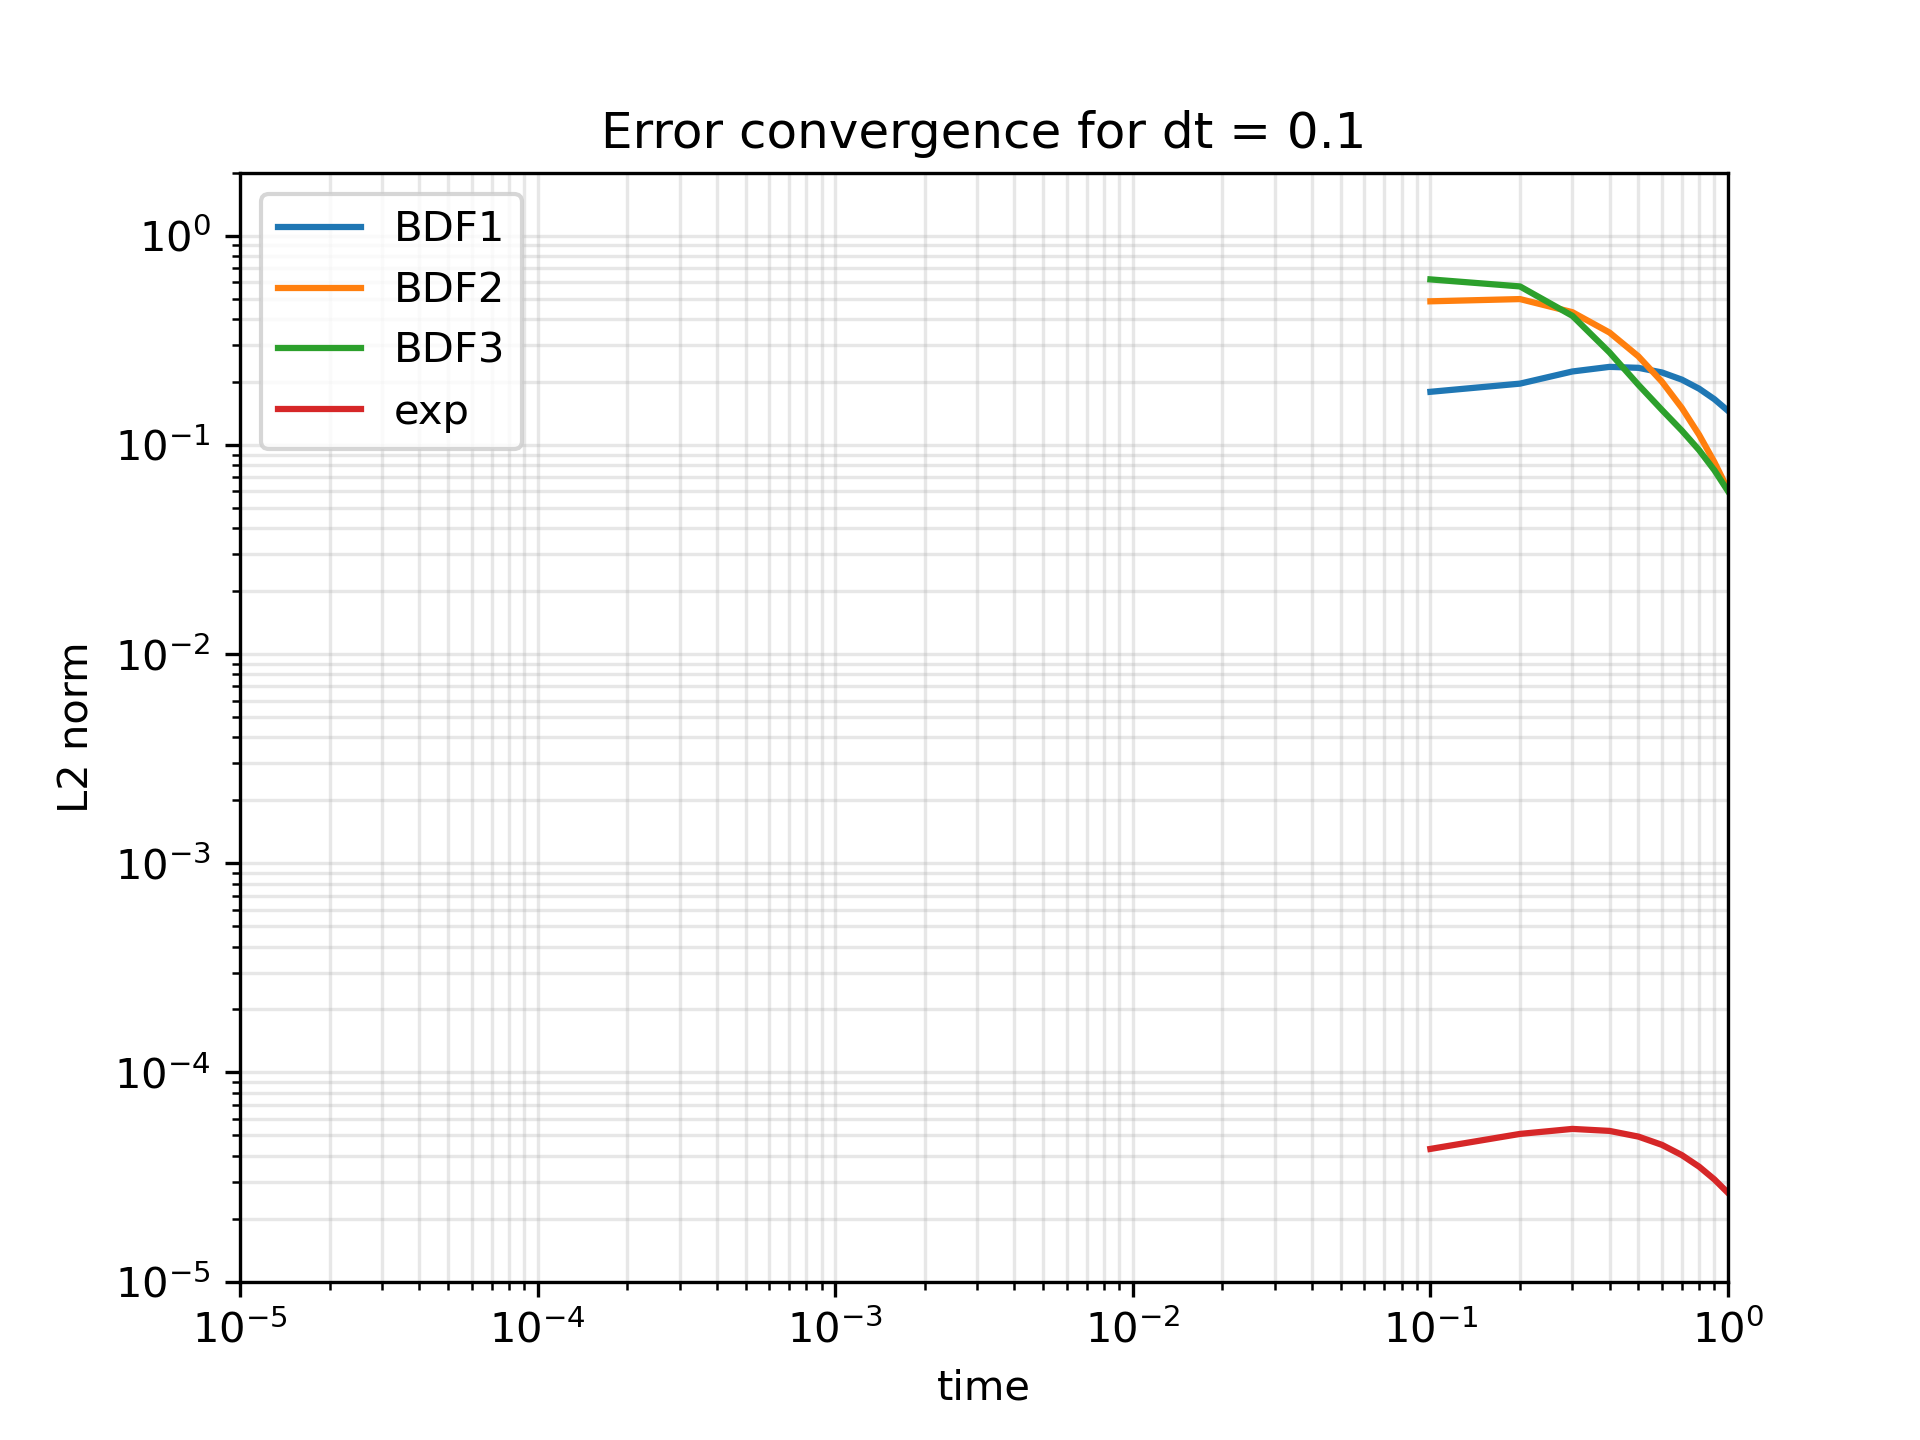
\includegraphics[width=0.7\linewidth]{res/no_homogeneo/L2norm_dt_0.1}
		\caption{}
		\label{fig:l2normdt0.1}
	\end{subfigure}
	\begin{subfigure}[b]{0.4\textwidth}
		\centering
		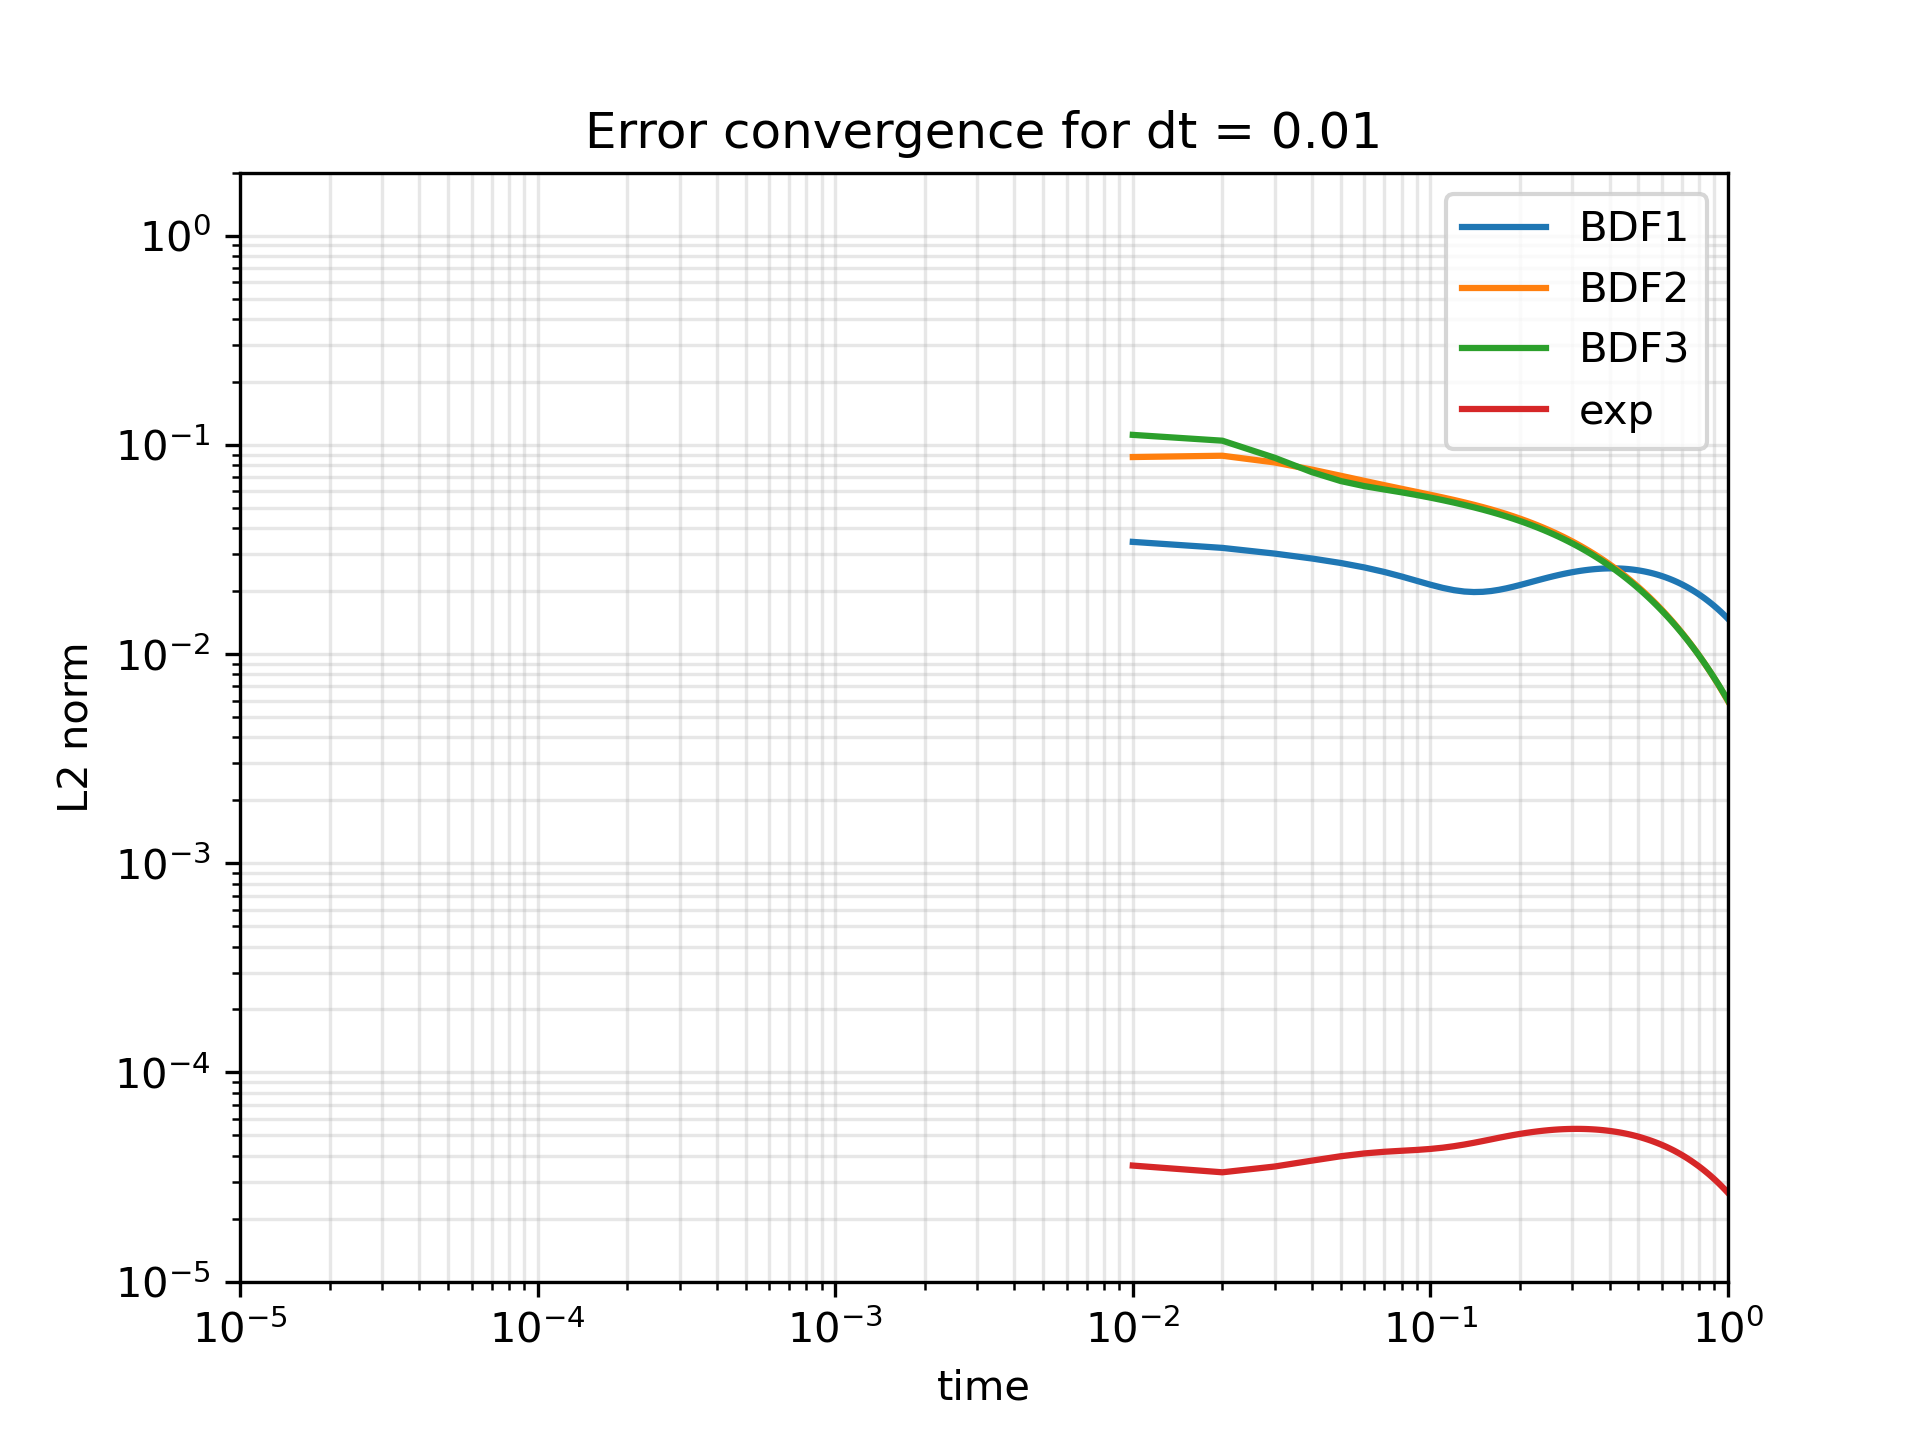
\includegraphics[width=0.7\linewidth]{res/no_homogeneo/L2norm_dt_0.01}
		\caption{}
		\label{fig:l2normdt0.01}
	\end{subfigure}
	\begin{subfigure}[b]{0.4\textwidth}
		\centering
		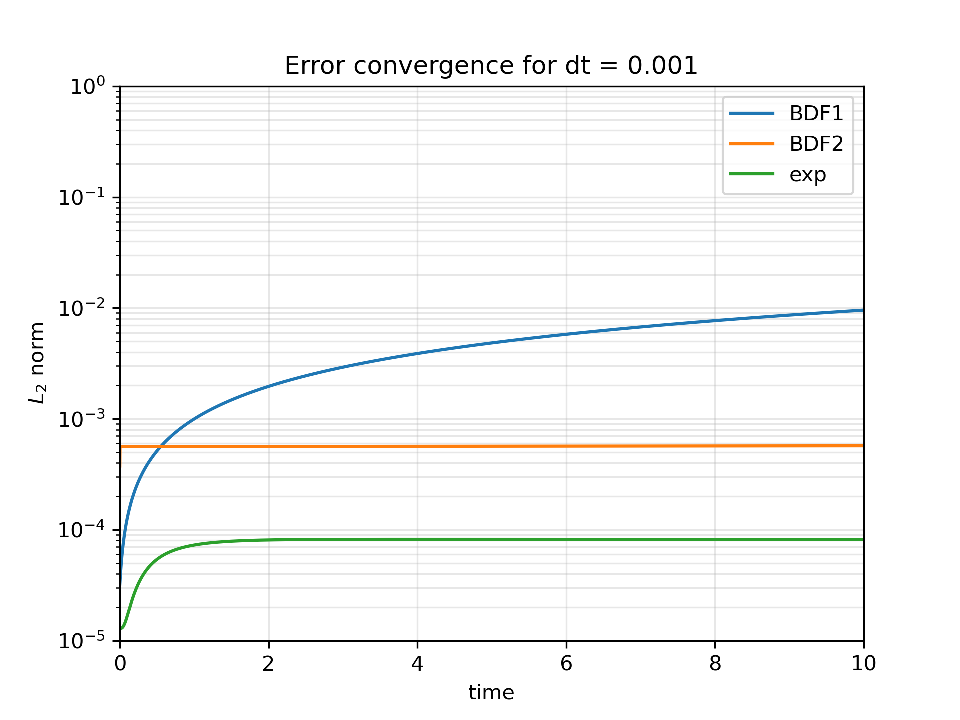
\includegraphics[width=0.7\linewidth]{res/no_homogeneo/L2norm_dt_0.001}
		\caption{}
		\label{fig:l2normdt0.001}
	\end{subfigure}
	\begin{subfigure}[b]{0.4\textwidth}
		\centering
		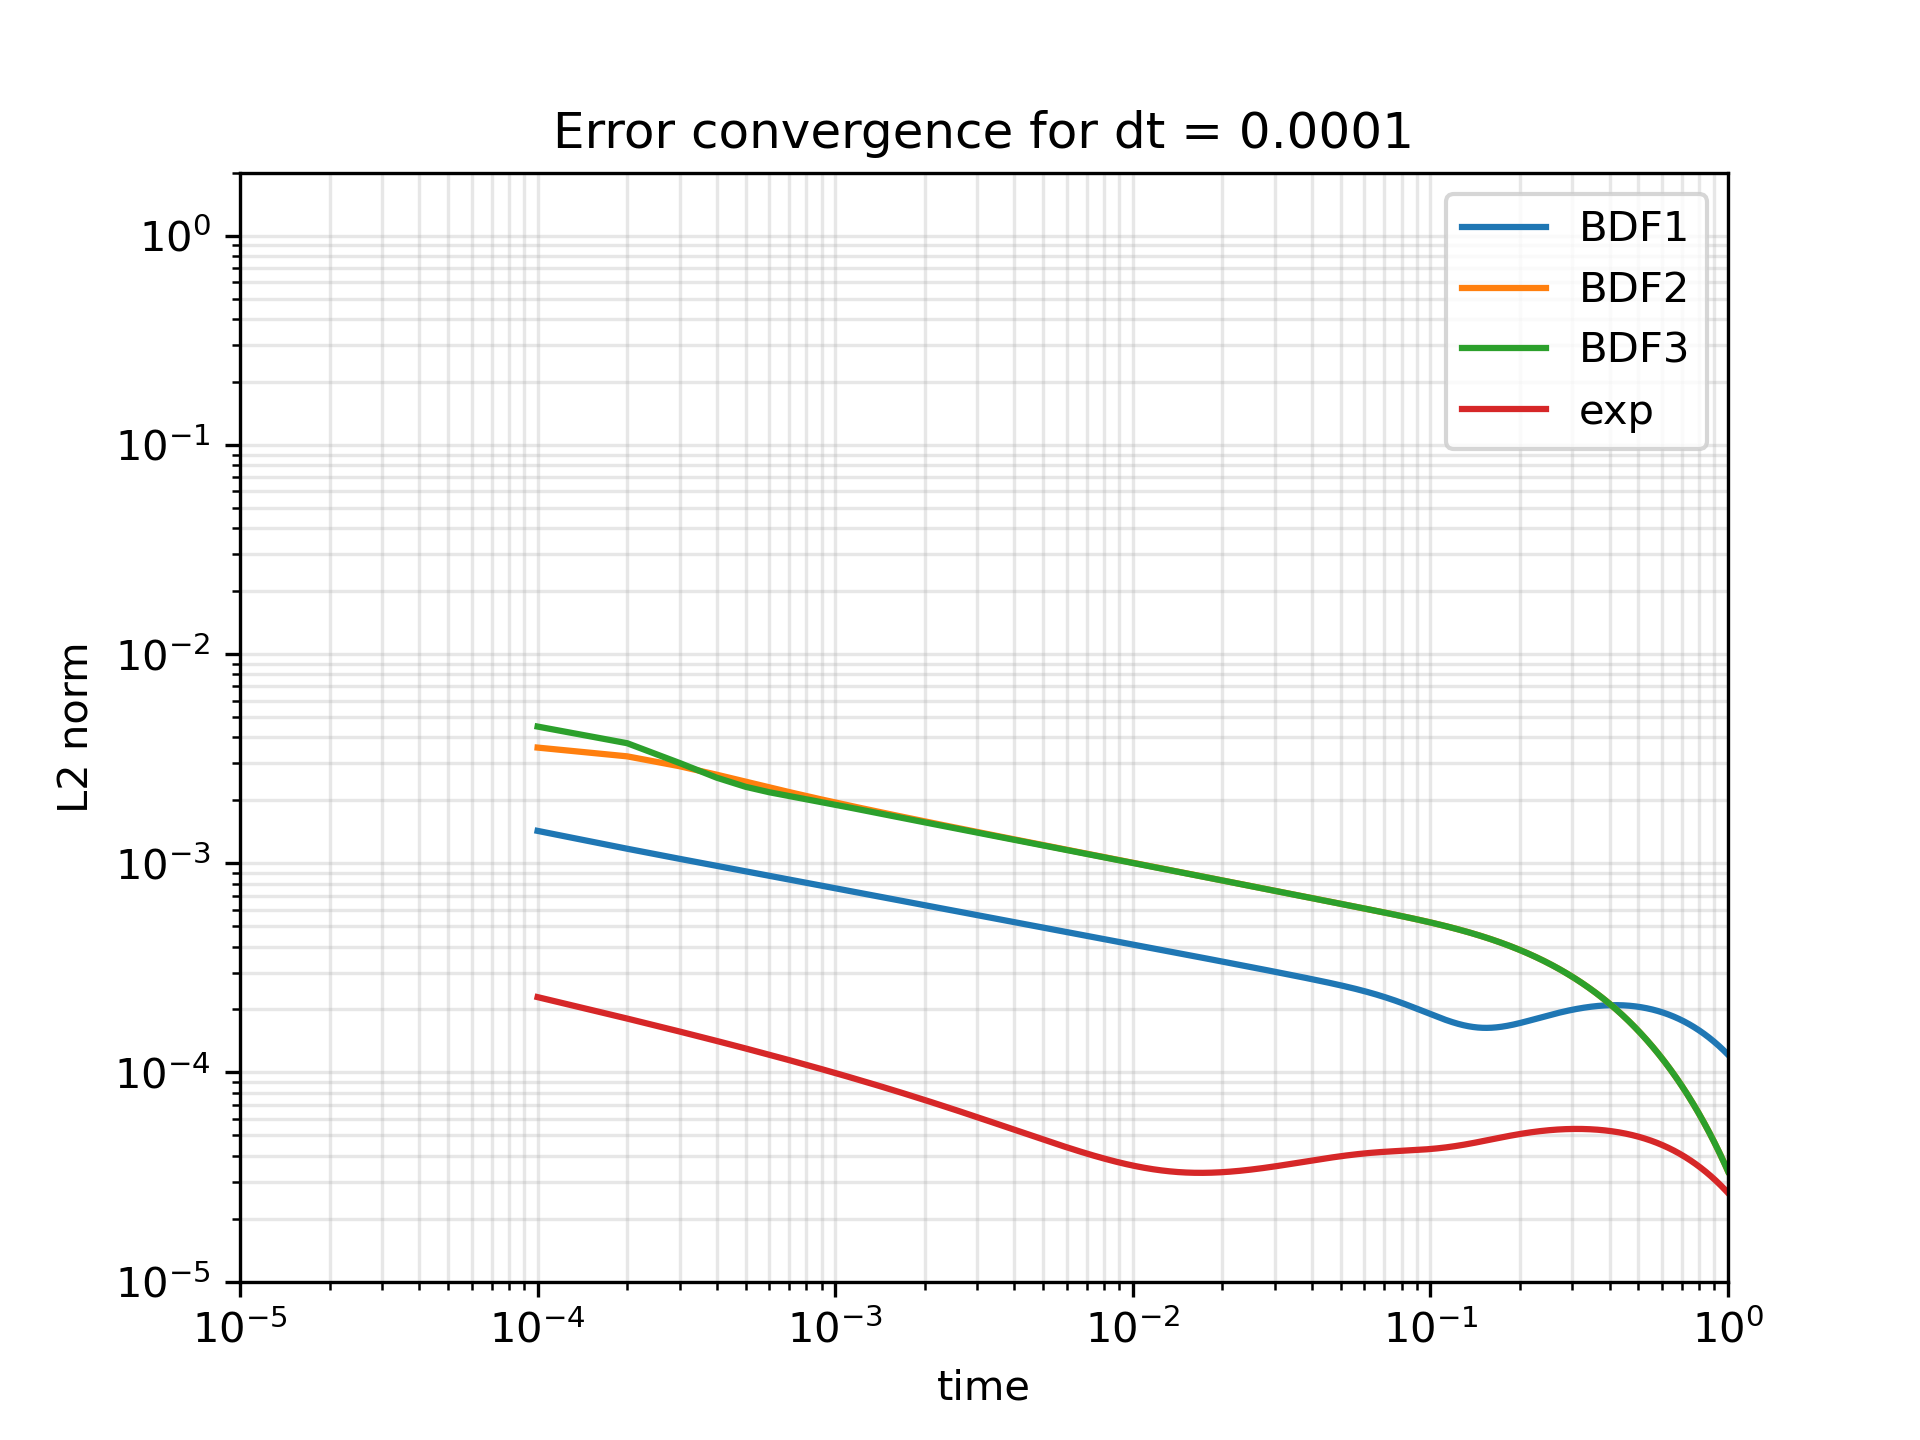
\includegraphics[width=0.7\linewidth]{res/no_homogeneo/L2norm_dt_0.0001}
		\caption{}
		\label{fig:l2normdt0.0001}
	\end{subfigure}
	\begin{subfigure}[b]{0.4\textwidth}
		\centering
		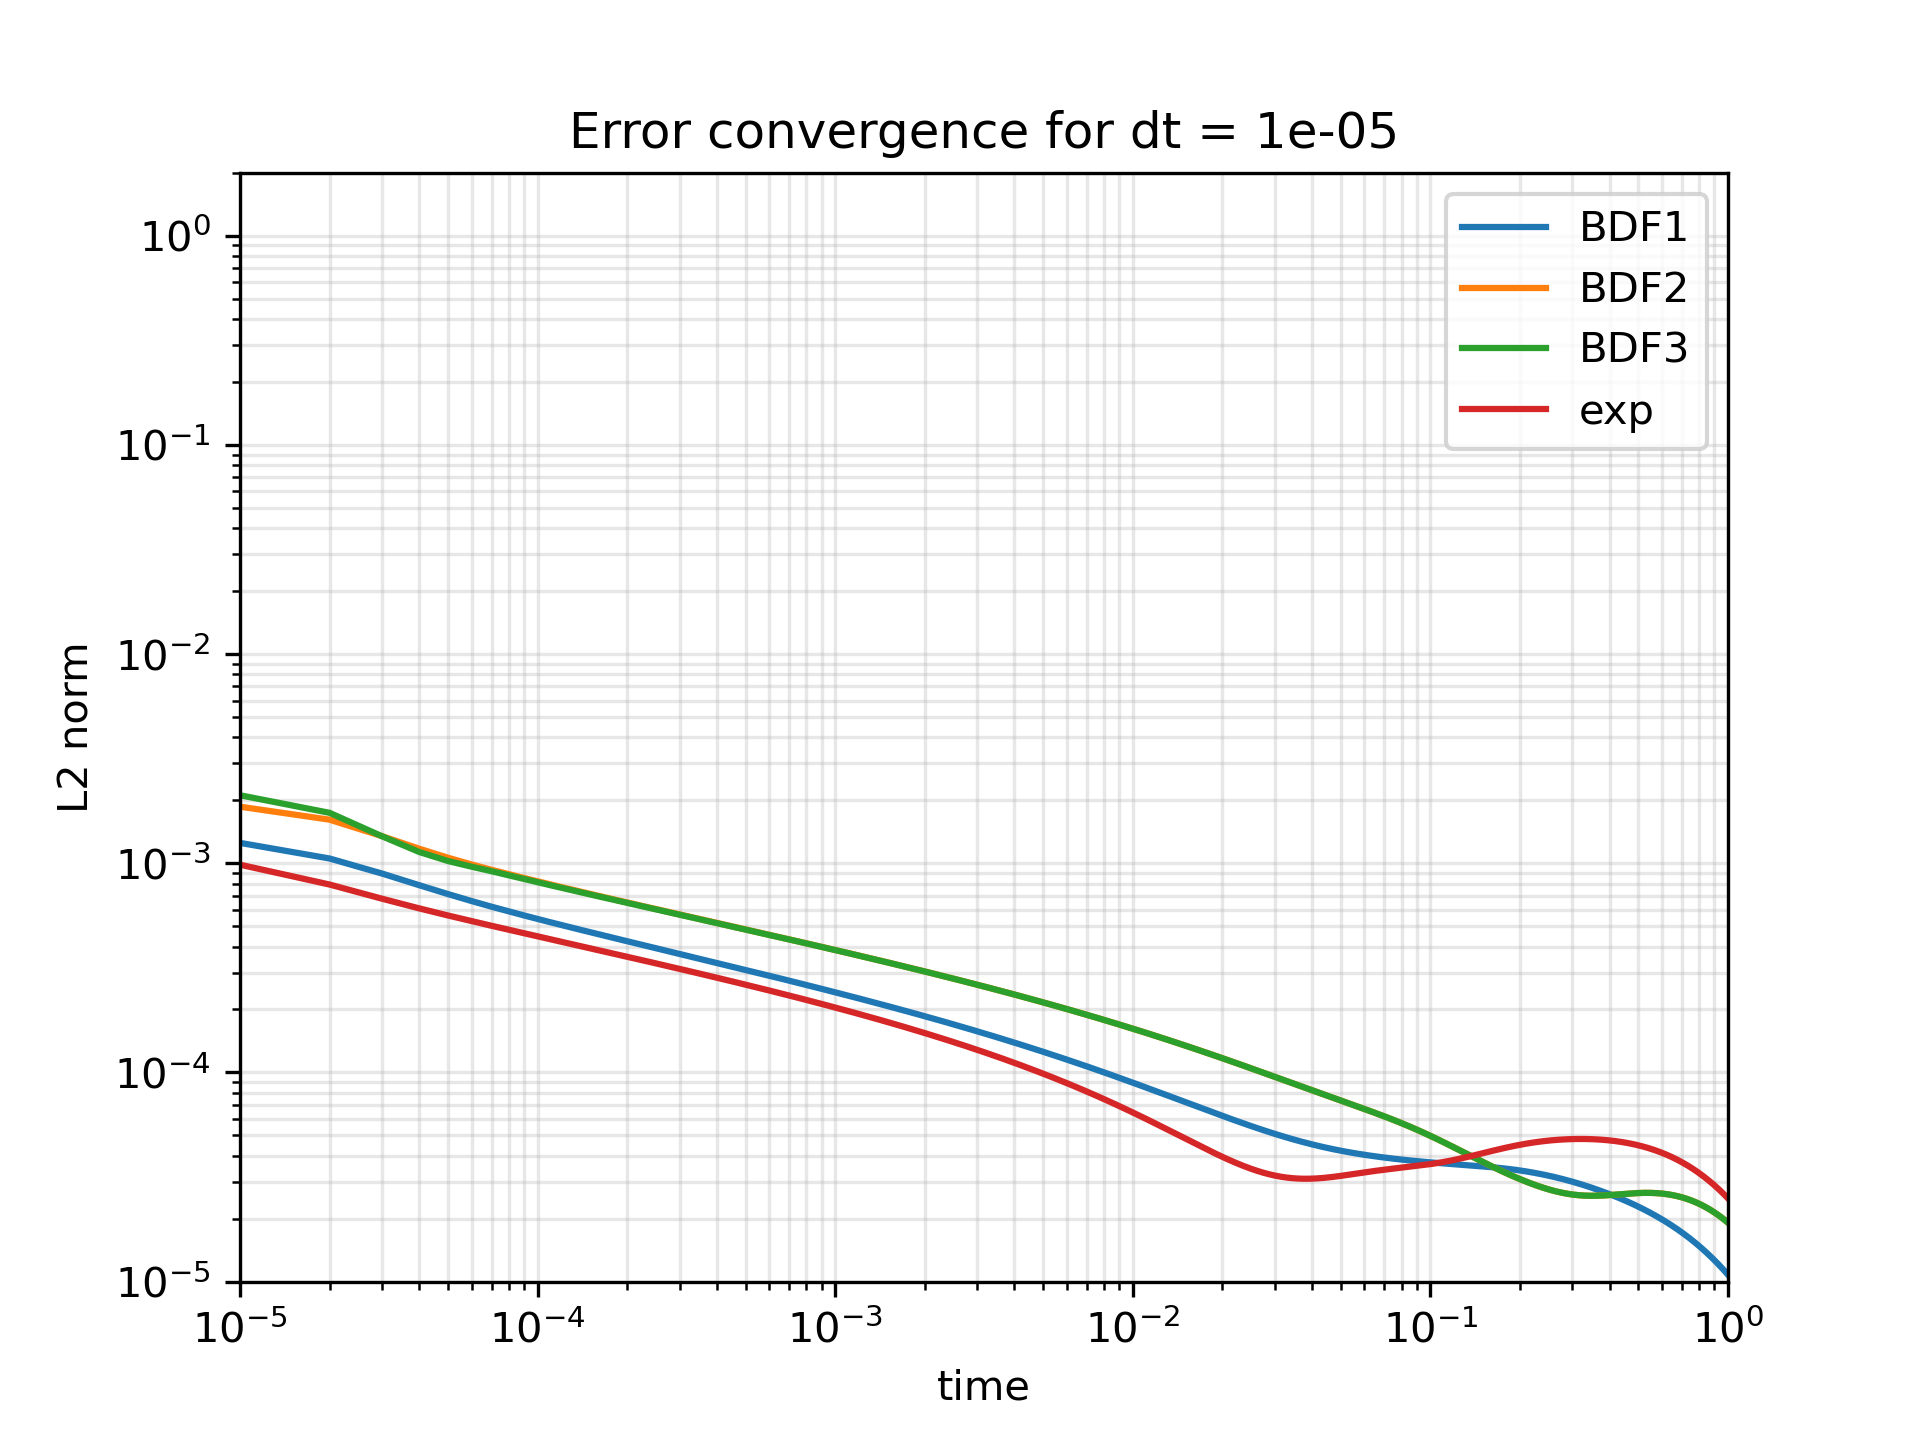
\includegraphics[width=0.7\linewidth]{res/no_homogeneo/L2norm_dt_1e-05.png}
		\caption{}
		\label{fig:l2normdt0.0001}
	\end{subfigure}
	\caption{Three simple graphs}
	\label{fig:three graphs}
\end{figure}

	




\begin{figure}
	\centering
	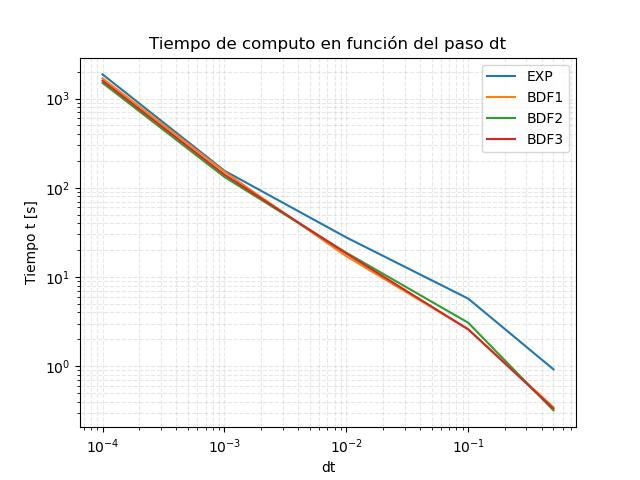
\includegraphics[width=0.7\linewidth]{res/no_homogeneo/tiempo_de_calculo}
	\caption{}
	\label{fig:tiempodecalculo}
\end{figure}

\begin{figure}[H]
	\centering
	\label{dominio del problema}
	\caption{dominio del problema}
	\begin{tikzpicture}[scale=2]
		
		% Dibujar el cuadrado
		\draw (0,0) --node[below]{T=0} (3,0) -- node[right]{T=0}  (3,3) --node[above]{q=0}  (0,3) -- node[left]{q=0} cycle;
		
		
		% Fuente en el interior
		\filldraw[fill=blue!20,draw=blue,thick] (1.5,1.5) circle [radius=0.07] node[right,black] {Q};
	\end{tikzpicture}
\end{figure}


	
\end{document}